\section{Evaluation} \label{evaluation}
When evaluating the success of a project, it is paramount to keep in mind the original intent of the project.
In this case, the primaray goal was to provide an alternative VM emulator implementation to the participants of the Nand to Tetris course to make Project 9 and 12 more convenient.
Not only was this goal achieved, but in addition, the CPU emulator was also rewritten and both emulators have been integrated into a test-script-driven workflow, making them useful to course instructors.
Then again, projects do not exist in a vaccum, so the following sections contain a comprehensive comparison with the official emulator.

\subsection{Web UI showcase} \label{ui-showcase}
The web based user interface is shown in~\cref{fig:ui-demo-desktop}. It is divided into four major parts.
Above everything else, there is a row with all interactive UI elements. It contains the buttons for loading a new program, starting, stopping, advancing a single step or resetting the running program and the slider for changing the VM execution speed.
In the middle left part of the screen the bytecode of the currently loaded program is displayed. This is useful when the user is using the ``Step'' button to debug the loaded program. The instruction to be executed next is highlighted in red.
To the right of that is the most important part of the user interface, the emulator screen.
Here the screen section of the emulator memory is displayed.
Below those two, certain parts of the internal memory are displayed to improve the debugging experience. From left to right, those are the call stack, local variables, arguments to the current function and the stack.
These fields are updated each time the emulator comes to a stop, i.e. after each step or after pressing the stop key. Since the emulator executes thousands of ticks per second, updating the values after each tick would be neither feasible nor useful.
The button row at the top and the screen are always visible.
In contrast, the bytecode view and the memory segments are hidden while the program is running. This allows the screen to fill almost the entire browser window and its contents to become as large as possible.
\begin{center}
  \begin{figure}[ht]
    \centering
    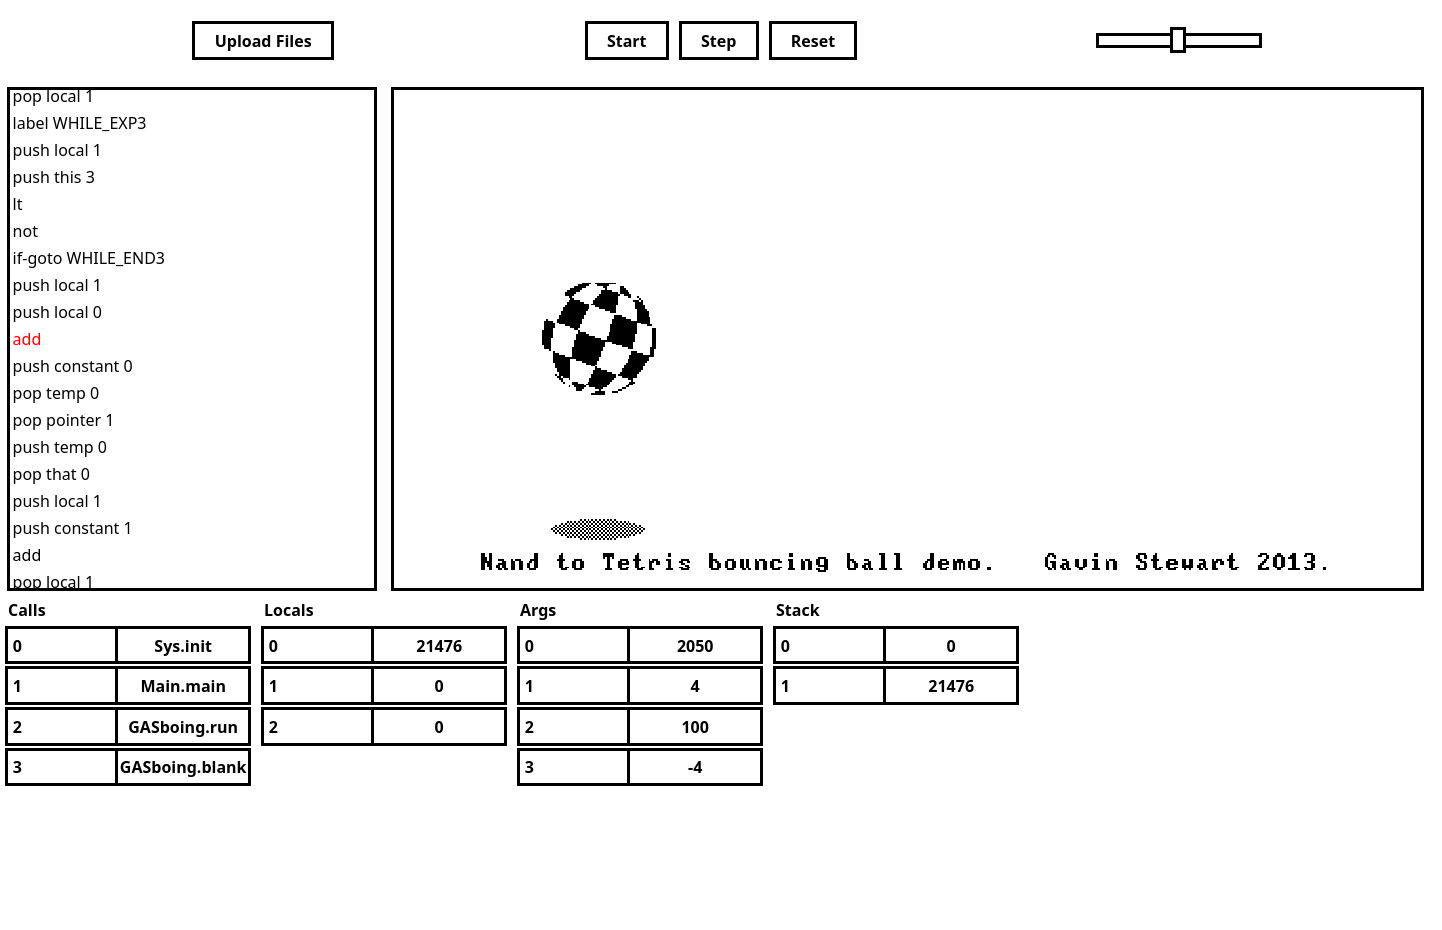
\includegraphics[width=12cm]{fig/ui-demo-desktop.png}
    \caption{The web based user interface on a desktop computer}%
    \label{fig:ui-demo-desktop}
  \end{figure}
\end{center}

\subsection{Comparison with the official Emulator based on compatability} \label{compatibility}
It is impossible to test every existing program for the Hack VM, both due to the sheer volume of existing applications and the fact that many of these applications are not available to the public.
However, this is also not necessary, since the expected behavior of the emulators is clearly described in the book that accompanies the course.
By following the specification and testing the new implementation with a reasonable number of representative programs, one can determine the degree of compatibility. Those programs are listed in the appendix~\ref{table:tested}.
The number of instructions in the VM is also manageable, so a sufficiently complex program will use every single available instruction, which further supports this claim.
By and large, the new emulator behaves exactly like the old one. This even applies to behaviors that could be considered bugs, such as the way the keyboard handler in the Java implementation interprets each letter as a capital letter, thus limiting the entire input system to uppercase letters.
This is not a technical limitation of either the VM or the Java input event, but simply a consequence of the implementation of the keyboard handler, and could easily be changed to allow lowercase letters as well.
However, this would break a number of existing applications as they only check for uppercase letters in their game code, meaning that these applications could no longer be used easily.
For this reason, the new emulator also only passes uppercase letters to the VM, even if it needs a bit more code to behave that way. All keys are converted directly to uppercase after being read.
In the future, it might be useful to add a compatibility setting to allow users to process lowercase letters as well, but due to time constraints in this project, it was decided to prioritize compatibility over correctness.
\label{sys.wait-compatibility}
There is only a single part of the new emulator that is known to behave at least partially differently to the official implementation. That is the implementation of the Sys.wait function, which was already discussed in detail in~\cref{sys.wait-example}.

% \begin{itemize}
%   \item every program working. systematic approach because there are tons of non public programs. Example programs that use every instruction/stdlib-function
%   \item Sys.wait not the same (but also different behaviour on official emulator, based on stdlib)
%   \item Sys.wait behaves differently in vm stdlib on official emulator
%   \item keyboard bug for bug compatible
% \end{itemize}

\subsection{Comparison with the official Emulator based on UI}
The new emulator does not implement all the features of the official emulator. Some of these missing features are missing due to time constraints, such as test script support in the WebUI~\ref{future-work}. On the other hand, some features have been deliberately omitted because they serve little purpose but complicate the user interface.
One such example is the ability to animate the running program. This may seem useful at first, but while debugging, the user will usually use the step button instead, and when running the game, the animations have to be disabled for performance reasons. So this feature does not provide any real value to the user.
Instead of offering every possible feature, the new user interface is intentionally kept minmal to simplify use and provide an experience that is more focused on actually running games at full speed. This is also the reason why most of the UI elements are completely hidden while the game is running.
For compiler development in projects 10 and 11, it may be advantageous to continue using the official emulators for their advanced debugging features.
On the contrary, when it comes to playing and testing full games, the new emulators offer a superior experience. They also open up these games and programs to additional platforms, because the new emulators also work on phones and tablets, as long as a physical keyboard is connected or the application does not require user input~\ref{fig:ui-demo-mobile}.
Another benefit of the new user interface is the unification of the VM and CPU emulators. The new emulator handles both types of applications within a single application, distinguishing between them based on their respective file extensions.
\begin{center}
  \begin{figure}[ht]
    \centering
    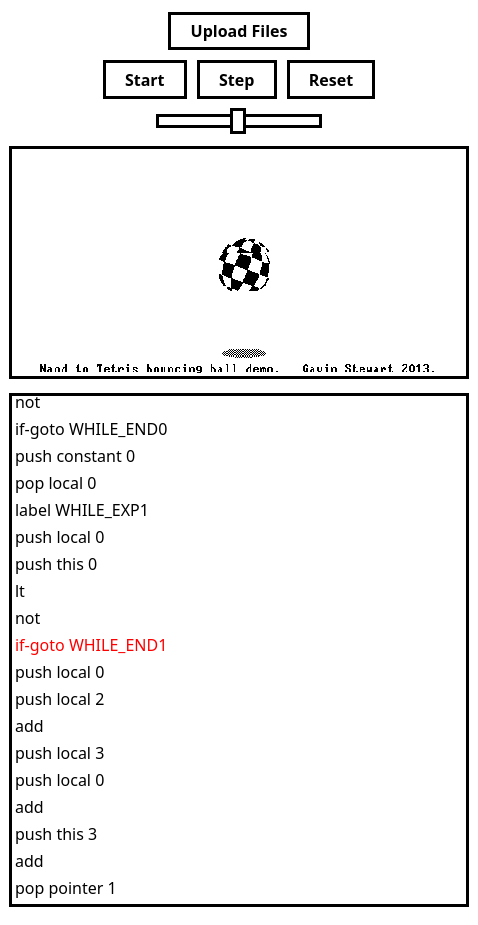
\includegraphics[width=6cm]{fig/ui-demo-mobile.png}
    \caption{The web based user interface in a phone format}%
    \label{fig:ui-demo-mobile}
  \end{figure}
\end{center}
% \begin{itemize}
%   \item official has more features (including test scripts)
%   \item mine scales better
%   \item mine is available in the browser -> also on mobile
%   \item mine handles cpu and vm in one ui
% \end{itemize}

\subsubsection{Hosting the application on GitHub Pages}
One of the biggest advantages of web-based applications is the ability to use them without a local installation, simply by opening a link in the user's web browser.
However, this only works if the application is hosted on a public web server. For many applications, this means renting or operating an expensive server infrastructure for the backend of their service.
In contrast, the new emulators are compiled to WebAssembly, which allows them to run entirely in the client's web browser. This means that no backend is needed and therefore a simple static file server is sufficient to host the entire application.
GitHub offers such a file hosting service free of charge. Users can simply upload their resources to a directory on GitHub's servers and mark that directory as public in the repository settings.
In addition, GitHub offers a service called ``GitHub Actions'' that allows arbitrary code to be executed on Microsoft's servers depending on various events in the respitory, such as a push to the main branch.
Combining these two services, one can automatically build and deploy the entire WebAssembly application to Pages every time there is a push to the main branch.
That is exactly what this project does, even though it is technically hosted on the HHU's internal GitLab instance.
Every time there is a push to the GitLab instance, that push is automatically mirrored to GitHub, which then builds the Wasm and JavaScript code and deploys it to GitHub Pages.

\subsection{Comparison with the official Emulator based on Performance} \label{sec:benchmarks}

There are two distinct modes in which the Emulators can operate: the interactive mode, in which the display memory is actually rendered to a visible canvas, and the test mode, in which a test scripts runs without any further user input to verify the correctness of a hack program.
From a performance point of view, however, only the former is relevant, since all test scripts used in the course finish so quickly that measuring the performance differences between different emulators would basically be meaningless.
So, to really evaluate the new emulators, a sufficiently complex graphical program is required. For this task, one of Gavin Stewart's impressive graphical demonstrations for the Hack platform was chosen.
The GASchunky program~\cite{demos} renders a complex animation in an infinite loop to the internal display. It requires no user input, but uses almost all of the available functionality of the platform, making it a perfect choice for benchmarking. In order to turn it into a proper benchmark, the loop was removed, leaving only a single iteration of the animation to be played.
\cref{fig:gaschunky-screenshot} shows a frame of the generated animation.
Additionally, to make the comparisons fair, all Sys.wait calls have been removed from the program. The reason why this is important was discussed in \cref{compatibility}.

Furthermore, some modifications were made to the emulators. For both the official and new graphical emualtors, two statements have been added to the code. Both print the current system time in milliseconds and get executed when the start button is pressed and when the program returns from the main function respectively. Additionally in the third column of the ~\cref{table:gaschunky}, the one millisecond wait instruction in the FastforwardTask of the HackController.java was removed to ensure that the official emulator could run at its maximum speed.
The new emulator was run both from the web UI and in desktop mode. In both cases the tickrate was set to one million, which is ten times as much as the normal maximum tickrate in the web UI. This limit is however arbitrarily chosen and therefore does not reflect the true performance of the system. At a tick rate of one million, the viewer can still see the animation clearly, which allows for a fair comparison.

\begin{table}[ht]
  \begin{center}
    \centering
    \begin{tabular}{@{}lllll@{}}
      \toprule
      Run & Official & Official (no wait) & Native &   Web \\ \midrule
      1   &   36.16s &             30.76s &  1.01s & 1.02s \\
      2   &   36.19s &             31.17s &  0.99s & 1.03s \\
      3   &   35.93s &             30.58s &  1.02s & 1.04s \\
      4   &   36.14s &             30.65s &  0.97s & 1.06s \\
      5   &   36.16s &             30.99s &  0.95s & 1.02s \\
      6   &   36.12s &             30.81s &  1.03s & 1.07s \\
      7   &   36.27s &             30.86s &  1.06s & 1.06s \\
      8   &   36.29s &             30.86s &  0.99s & 1.05s \\
      9   &   35.86s &             30.81s &  1.01s & 1.03s \\
      10  &   36.12s &             30.74s &  1.02s & 1.04s \\ \bottomrule
    \end{tabular}
    \caption{GASchunky benchmark (lower is faster)}%
    \label{table:gaschunky}
  \end{center}
\end{table}

\begin{figure}[ht]
  \centering
  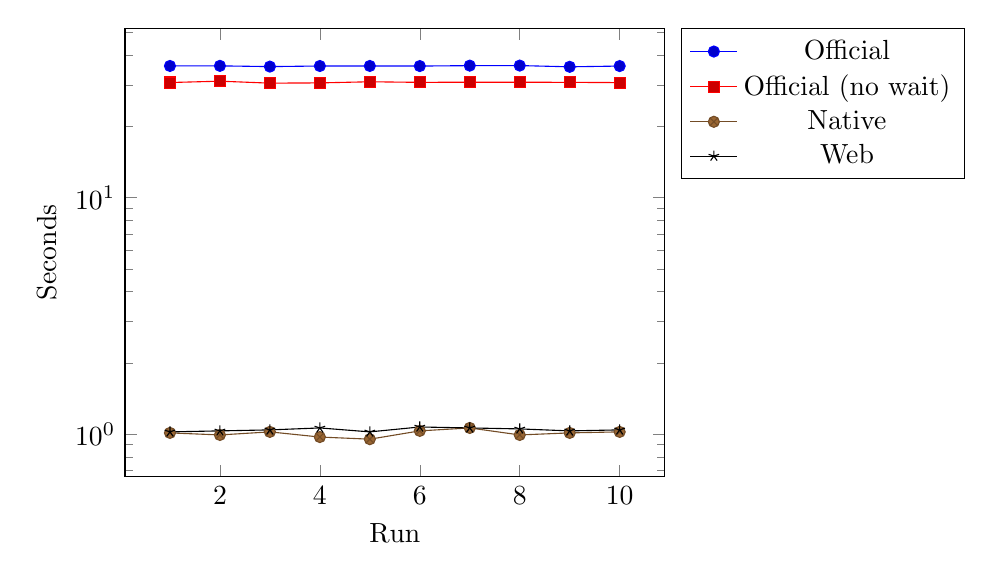
\begin{tikzpicture}
    \begin{axis}[
      ymode=log,
      ylabel=Seconds,
      xlabel=Run,
      legend pos=outer north east,
      ]
      \addplot coordinates {
        (1,  36.16)
        (2,  36.19)
        (3,  35.93)
        (4,  36.14)
        (5,  36.16)
        (6,  36.12)
        (7,  36.27)
        (8,  36.29)
        (9,  35.86)
        (10, 36.12)
      };
      \addplot coordinates {
        (1,  30.76)
        (2,  31.17)
        (3,  30.58)
        (4,  30.65)
        (5,  30.99)
        (6,  30.81)
        (7,  30.86)
        (8,  30.86)
        (9,  30.81)
        (10, 30.74)
      };
      \addplot coordinates {
        (1,  1.01)
        (2,  0.99)
        (3,  1.02)
        (4,  0.97)
        (5,  0.95)
        (6,  1.03)
        (7,  1.06)
        (8,  0.99)
        (9,  1.01)
        (10, 1.02)
      };
      \addplot coordinates {
        (1,  1.02)
        (2,  1.03)
        (3,  1.04)
        (4,  1.06)
        (5,  1.02)
        (6,  1.07)
        (7,  1.06)
        (8,  1.05)
        (9,  1.03)
        (10, 1.04)
      };
      \addlegendentry{Official}
      \addlegendentry{Official (no wait)}
      \addlegendentry{Native}
      \addlegendentry{Web}
    \end{axis}
  \end{tikzpicture}
  \caption{GASchunky benchmark (lower is faster)}%
  \label{fig:gachunky-plot}
\end{figure}

It is clearly visible that the new Emulator is several times faster than the official implementation.
On average, the official emulator without modifications takes around 36 seconds to render the full animation once. Meanwhile the Web version of the new emulator manages to achieve the same result in just one second on average. The native version of the new emulator which uses SDL to render the internal display is even slightly faster. While the official emulator can be sped up drastically, it still does not come close.
This shows us that even though the new emulator only uses a single thread and runs in a browser, it still offers massive performance benefits over the official implementation.

\begin{center}
  \begin{figure}[ht]
    \centering
    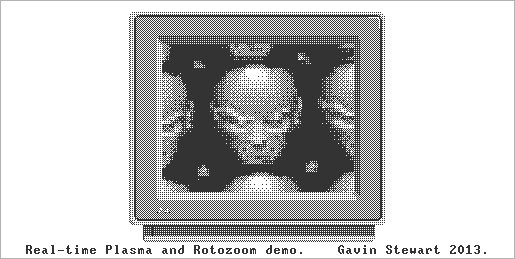
\includegraphics[width=10cm]{fig/gaschunky.png}
    \caption{A screenshot of the GASchunky animation in progress}%
    \label{fig:gaschunky-screenshot}
  \end{figure}
\end{center}
